

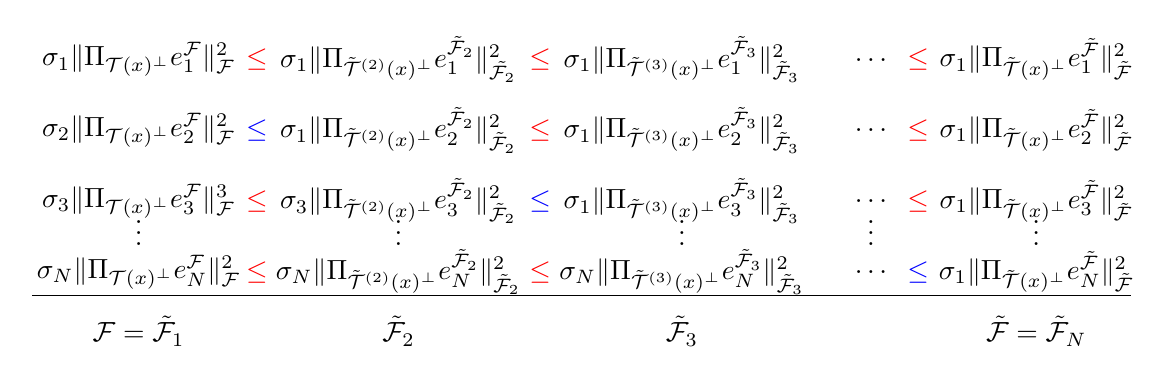
\begin{tikzpicture}[scale = 0.3]

  % draw line and angle
%  \draw 
%     pic [draw,angle radius=4mm,angle eccentricity=1.5, "$\theta$" font=\scriptsize] {angle=v2--v1--v3};

 

%\draw [fill=blue, opacity=0.5] (-15,3.75) -- (-11,3.75) -- (-11,5.5) -- (-15,5.5) -- (-15,3.75);
%\draw [fill=blue, opacity=0.5] (-15,3.5) -- (-11,3.5) -- (-11,3.75) -- (-15,3.75) -- (-15,3.5);
%\draw [fill=blue, opacity=0.5] (-15,3.25) -- (-11,3.25) -- (-11,3.5) -- (-15,3.5) -- (-15,3.25);
%\draw [fill=blue, opacity=0.5] (-15,4) -- (-11,4) -- (-11,3.25) -- (-15,3.25) -- (-15,4);
%\draw [fill=blue, opacity=0.5] (-15,2.75) -- (-11,2.75) -- (-11,4) -- (-15,4) -- (-15,2.75); 
%\draw [fill=blue, opacity=0.5] (-15,2.5) -- (-11,2.5) -- (-11,2.75) -- (-15,2.75) -- (-15,2.5);
%\draw [fill=blue, opacity=0.5] (-15,2.25) -- (-11,2.25) -- (-11,2.5) -- (-15,2.5) -- (-15,2.25);
%\draw [fill=blue, opacity=0.5] (-15,2) -- (-11,2) -- (-11,2.25) -- (-15,2.25) -- (-15,2);
%\draw [fill=blue, opacity=0.5] (-15,1.75) -- (-11,1.75) -- (-11,2) -- (-15,2) -- (-15,1.75);



%\draw [fill=blue, opacity=1] (-2,3.75) -- (2,3.75) -- (2,5.5) -- (-2,5.5) -- (-2,3.75);
%\draw [fill=blue, opacity=1] (-2,3.5) -- (2,3.5) -- (2,3.75) -- (-2,3.75) -- (-2,3.5);
%\draw [fill=blue, opacity=0.5] (-2,3.25) -- (2,3.25) -- (2,3.5) -- (-2,3.5) -- (-2,3.25);
%\draw [fill=blue, opacity=0.5] (-2,4) -- (2,4) -- (2,3.25) -- (-2,3.25) -- (-2,4);
%\draw [fill=blue, opacity=1] (-2,2.75) -- (2,2.75) -- (2,4) -- (-2,4) -- (-2,2.75); 
%\draw [fill=blue, opacity=0.5] (-2,2.5) -- (2,2.5) -- (2,2.75) -- (-2,2.75) -- (-2,2.5);
%\draw [fill=blue, opacity=0.5] (-2,2.25) -- (2,2.25) -- (2,2.5) -- (-2,2.5) -- (-2,2.25);
%\draw [fill=blue, opacity=1] (-2,2) -- (2,2) -- (2,2.25) -- (-2,2.25) -- (-2,2);
%\draw [fill=blue, opacity=0.5] (-2,1.75) -- (2,1.75) -- (2,2) -- (-2,2) -- (-2,1.75);





%\draw [fill=blue, opacity=1] (13,2.75) -- (17,2.75) -- (17,4) -- (13,4) -- (13,2.75);
%\draw [fill=blue, opacity=1] (13,2.5) -- (17,2.5) -- (17,2.75) -- (13,2.75) -- (13,2.5);
%\draw [fill=blue, opacity=1] (13,2.25) -- (17,2.25) -- (17,2.5) -- (13,2.5) -- (13,2.25);
%\draw [fill=blue, opacity=1] (13,2) -- (17,2) -- (17,2.25) -- (13,2.25) -- (13,2);


%\draw [fill=orange, opacity=1] (13.25,2) -- (13.25,2) -- (13.5,2) -- (13.5,4) -- (13.25,4);
%\draw [fill=orange, opacity=1] (14.25,2) -- (14.25,2) -- (14.5,2) -- (14.5,4) -- (14.25,4);
%\draw [fill=orange, opacity=1] (14.75,2) -- (14.75,2) -- (15,2) -- (15,4) -- (14.75,4);
%\draw [fill=orange, opacity=1] (15.75,2) -- (15.75,2) -- (16,2) -- (16,4) -- (15.75,4);



%\draw [->] (-7.5,2) --  (-6.5,2)  node [above] {\tiny $\Prb(T) \propto \prod_{i \in T} \sigma_{i}^{2}$} --  (-5.5,2);

%\draw [->] (6.5,2) --  (7.5,2)  node [above] {\tiny $\Prb(S|T) = \Det (\bm{V}_{S,T})^{2}$} --  (11.5,2);

%\draw  (-17,2.25)  node [above] {$\bm{V}^{\Tran}=$} ;

\draw  (-43,7)  node  {$\sigma_{1}\|\bm{\Pi}_{\mathcal{T}(\bm{x})^{\perp}}e_{1}^{\mathcal{F}}\|^{2}_{\mathcal{F}}$} ;
\draw  (-38,7)  node  {$\color{red} \leq$} ;
\draw  (-32,7)  node  {$\sigma_{1}\|\bm{\Pi}_{\tilde{\mathcal{T}}^{(2)}(\bm{x})^{\perp}}e_{1}^{\tilde{\mathcal{F}}_{2}}\|^{2}_{\tilde{\mathcal{F}_{2}}}$} ;
\draw  (-26,7)  node  {$\color{red} \leq$} ;
\draw  (-20,7)  node  {$\sigma_{1}\|\bm{\Pi}_{\tilde{\mathcal{T}}^{(3)}(\bm{x})^{\perp}}e_{1}^{\tilde{\mathcal{F}}_{3}}\|^{2}_{\tilde{\mathcal{F}}_{3}}$} ;
%\draw  (-20,7)  node  {$\leq$} ;
\draw  (-12,7)  node  {$\dots$} ;

\draw  (-10,7)  node  {$\color{red} \leq$} ;
\draw  (-5,7)  node  {$\sigma_{1}\|\bm{\Pi}_{\tilde{\mathcal{T}}(\bm{x})^{\perp}}e_{1}^{\tilde{\mathcal{F}}}\|^{2}_{\tilde{\mathcal{F}}}$} ;




\draw  (-43,4)  node  {$\sigma_{2}\|\bm{\Pi}_{\mathcal{T}(\bm{x})^{\perp}}e_{2}^{\mathcal{F}}\|^{2}_{\mathcal{F}}$} ;
\draw  (-38,4)  node  {$\color{blue} \leq$} ;
\draw  (-32,4)  node  {$\sigma_{1}\|\bm{\Pi}_{\tilde{\mathcal{T}}^{(2)}(\bm{x})^{\perp}}e_{2}^{\tilde{\mathcal{F}}_{2}}\|^{2}_{\tilde{\mathcal{F}}_{2}}$} ;
\draw  (-26,4)  node  {$\color{red} \leq$} ;
\draw  (-20,4)  node  {$\sigma_{1}\|\bm{\Pi}_{\tilde{\mathcal{T}}^{(3)}(\bm{x})^{\perp}}e_{2}^{\tilde{\mathcal{F}}_{3}}\|^{2}_{\tilde{\mathcal{F}}_{3}}$} ;
%\draw  (-20,7)  node  {$\leq$} ;
\draw  (-12,4)  node  {$\dots$} ;

\draw  (-10,4)  node  {$\color{red} \leq$} ;
\draw  (-5,4)  node  {$\sigma_{1}\|\bm{\Pi}_{\tilde{\mathcal{T}}(\bm{x})^{\perp}}e_{2}^{\tilde{\mathcal{F}}}\|^{2}_{\tilde{\mathcal{F}}}$} ;


\draw  (-43,1)  node  {$\sigma_{3}\|\bm{\Pi}_{\mathcal{T}(\bm{x})^{\perp}}e_{3}^{\mathcal{F}}\|^{3}_{\mathcal{F}}$} ;
\draw  (-38,1)  node  {$\color{red} \leq$} ;
\draw  (-32,1)  node  {$\sigma_{3}\|\bm{\Pi}_{\tilde{\mathcal{T}}^{(2)}(\bm{x})^{\perp}}e_{3}^{\tilde{\mathcal{F}}_{2}}\|^{2}_{\tilde{\mathcal{F}}_{2}}$} ;
\draw  (-26,1)  node  {$\color{blue} \leq$} ;
\draw  (-20,1)  node  {$\sigma_{1}\|\bm{\Pi}_{\tilde{\mathcal{T}}^{(3)}(\bm{x})^{\perp}}e_{3}^{\tilde{\mathcal{F}}_{3}}\|^{2}_{\tilde{\mathcal{F}}_{3}}$} ;
%\draw  (-20,7)  node  {$\leq$} ;
\draw  (-12,1)  node  {$\dots$} ;

\draw  (-10,1)  node  {$\color{red} \leq$} ;
\draw  (-5,1)  node  {$\sigma_{1}\|\bm{\Pi}_{\tilde{\mathcal{T}}(\bm{x})^{\perp}}e_{3}^{\tilde{\mathcal{F}}}\|^{2}_{\tilde{\mathcal{F}}}$} ;


\draw  (-43,0)  node  {$\vdots$} ;
%\draw  (-36,0)  node  {$\leq$} ;
\draw  (-32,0)  node  {$\vdots$} ;
%\draw  (-28,0)  node  {$\leq$} ;
\draw  (-20,0)  node  {$\vdots$} ;
%\draw  (-20,7)  node  {$\leq$} ;
\draw  (-12,0)  node  {$\vdots$} ;

%\draw  (-12,0)  node  {$\leq$} ;
\draw  (-5,0)  node  {$\vdots$} ;



\draw  (-43,-2)  node  {$\sigma_{N}\|\bm{\Pi}_{\mathcal{T}(\bm{x})^{\perp}}e_{N}^{\mathcal{F}}\|^{2}_{\mathcal{F}}$} ;
\draw  (-38,-2)  node  {$\color{red} \leq$} ;
\draw  (-32,-2)  node  {$\sigma_{N}\|\bm{\Pi}_{\tilde{\mathcal{T}}^{(2)}(\bm{x})^{\perp}}e_{N}^{\tilde{\mathcal{F}}_{2}}\|^{2}_{\tilde{\mathcal{F}}_{2}}$} ;
\draw  (-26,-2)  node  {$\color{red} \leq$} ;
\draw  (-20,-2)  node  {$\sigma_{N}\|\bm{\Pi}_{\tilde{\mathcal{T}}^{(3)}(\bm{x})^{\perp}}e_{N}^{\tilde{\mathcal{F}}_{3}}\|^{2}_{\tilde{\mathcal{F}}_{3}}$} ;
%\draw  (-20,7)  node  {$\leq$} ;
\draw  (-12,-2)  node  {$\dots$} ;

\draw  (-10,-2)  node  {$\color{blue} \leq$} ;
\draw  (-5,-2)  node  {$\sigma_{1}\|\bm{\Pi}_{\tilde{\mathcal{T}}(\bm{x})^{\perp}}e_{N}^{\tilde{\mathcal{F}}}\|^{2}_{\tilde{\mathcal{F}}}$} ;

\draw[line width=0.15 mm] (-47.5,-3) -- (-1,-3);

\draw  (-43,-4.5)  node  {$\mathcal{F}=\tilde{\mathcal{F}}_{1}$} ;
\draw  (-38,-4.5)  node  {} ;
\draw  (-32,-4.5)  node  {$\tilde{\mathcal{F}}_{2}$} ;
\draw  (-26,-4.5)  node  {} ;
\draw  (-20,-4.5)  node  {$\tilde{\mathcal{F}}_{3}$} ;
%\draw  (-20,7)  node  {$\leq$} ;
\draw  (-12,-4.5)  node  {} ;

\draw  (-10,-4.5)  node  {} ;
\draw  (-5,-4.5)  node  {$\tilde{\mathcal{F}} = \tilde{\mathcal{F}}_{N}$} ;
\end{tikzpicture}
